\chapter{Background}\label{chap:Fondamenti Teorici}

\section{Introduzione a Kubernetes}

Kubernetes\footnote{https://kubernetes.io}, spesso abbreviato come K8s, è un sistema open source che permette di automatizzare il deployment, la scalabilità e la gestione di applicazioni containerizzate. Kubernetes fornisce un ambiente di esecuzione distribuito e robusto per applicazioni, offrendo un'alternativa più efficiente e flessibile rispetto alla gestione manuale dei container.

\subsection{Architettura di Kubernetes}

L'architettura di Kubernetes è costituita da un cluster che include almeno un nodo \textit{master} e uno o più nodi \textit{worker}. Il nodo \textit{master} coordina il cluster, mentre i nodi \textit{worker} eseguono le applicazioni (\textit{Figura \ref{fig:kube_components}}).

\subsubsection{Nodo master}
Il nodo master ospita diversi componenti che costituiscono il \textit{control plane} di Kubernetes. Questi componenti includono:

\begin{itemize}
\item \textit{API Server}: È il punto di ingresso per tutte le API RESTful di Kubernetes. Gestisce le operazioni di lettura e scrittura nel database del cluster e controlla l'accesso alle risorse del cluster.
\item \textit{Controller Manager}: Esegue i \textit{controller}, ovvero i processi di background che gestiscono lo stato del cluster. I \textit{controller} includono il \textit{Node Controller}, \textit{Replication Controller}, \textit{Endpoints Controller} e \textit{Service Account \& Token Controllers}.
\item \textit{Scheduler}: Assegna i pod (gruppi di uno o più container) ai nodi \textit{worker} in base ai requisiti di risorse e altre precise restrizioni.
\item \textit{etcd}: È un sistema di memorizzazione di dati distribuito e persistente che permette di salvare l'intero stato del cluster.
\end{itemize}
\subsubsection{Nodo worker}
I nodi \textit{worker}, facenti parte del \textit{data plane} di Kubernetes, ospitano i pod che eseguono le applicazioni. Ogni nodo \textit{worker} include i seguenti componenti:

\begin{itemize}
\item \textit{Kubelet}: È l'agente che è eseguito su ogni nodo e che si assicura che i container siano in esecuzione in un pod.
\item \textit{Kube-proxy}: Gestisce il networking dei pod, permettendo la comunicazione di rete ai pod da rete esterna e viceversa.
\end{itemize}

\begin{figure}[h]
    \centering
    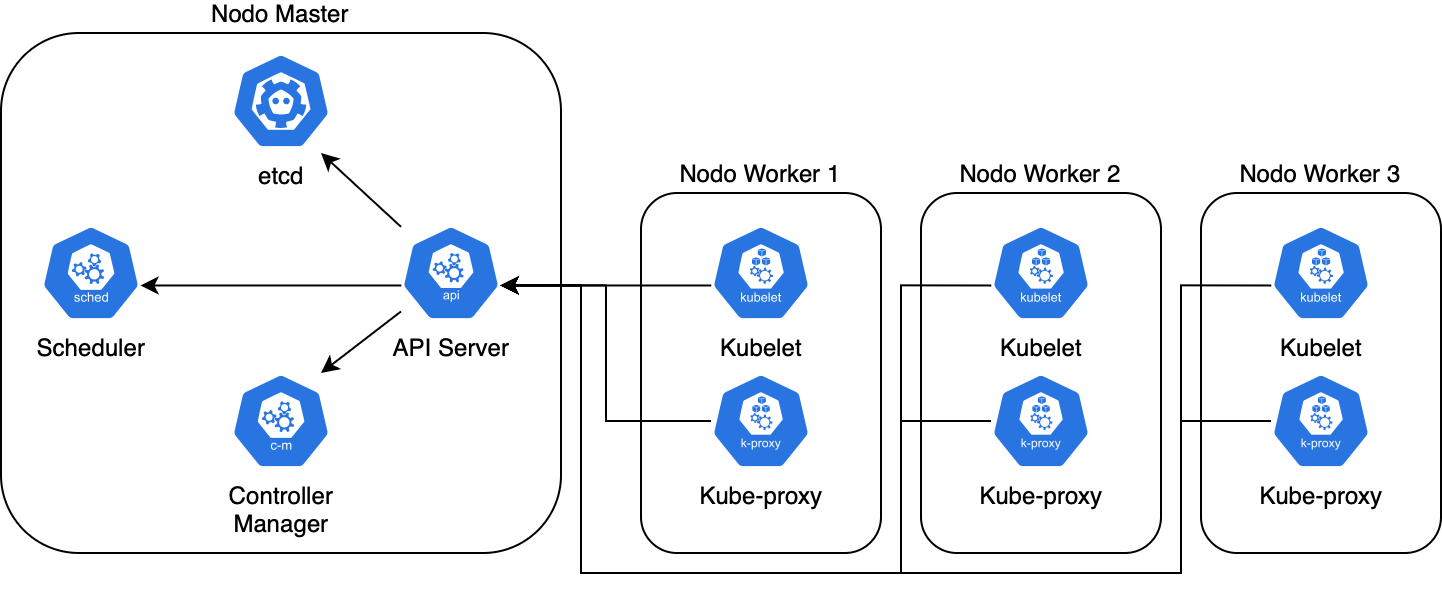
\includegraphics[width=1\linewidth]{immagini/capitolo2/kubernetes_planes.png}
    \caption{Organizzazione dei componenti Kubernetes.}
    \label{fig:kube_components}
\end{figure}

\subsection{Risorse di Kubernetes}

Kubernetes gestisce le applicazioni attraverso vari tipi di risorse, ognuna delle quali possiede un ruolo specifico:

\begin{itemize}
\item \textit{Pod}: È la più piccola e semplice unità in Kubernetes. Un Pod rappresenta una singola istanza di un microservizio e può contenere uno o più container.
\item \textit{Service}: È un'astrazione che definisce un insieme logico di Pod e la politica di accesso a essi.
\item \textit{Volume}: Fornisce storage persistente per i container in un Pod.
\item \textit{Namespace}: Permette di dividere le risorse di un cluster fisico in più cluster virtuali. Ogni namespace fornisce lo scope per i nomi delle risorse.
\item \textit{Deployment}: Permette di descrivere lo stato desiderato per i Pod o i ReplicaSet. Il Deployment Controller cambia lo stato attuale allo stato desiderato a un ritmo controllato.
\item \textit{ConfigMap} e \textit{Secret}: Forniscono meccanismi per iniettare configurazione e dati sensibili, rispettivamente, nei container.
\item \textit{Ingress}: È un'API che gestisce l'accesso esterno ai servizi in un cluster, tipicamente HTTP.
\end{itemize}
La Figura \ref{fig:kube_objects} mostra l'organizzazione delle risorse all'interno di un cluster Kubernetes.
\begin{figure}[h]
    \centering
    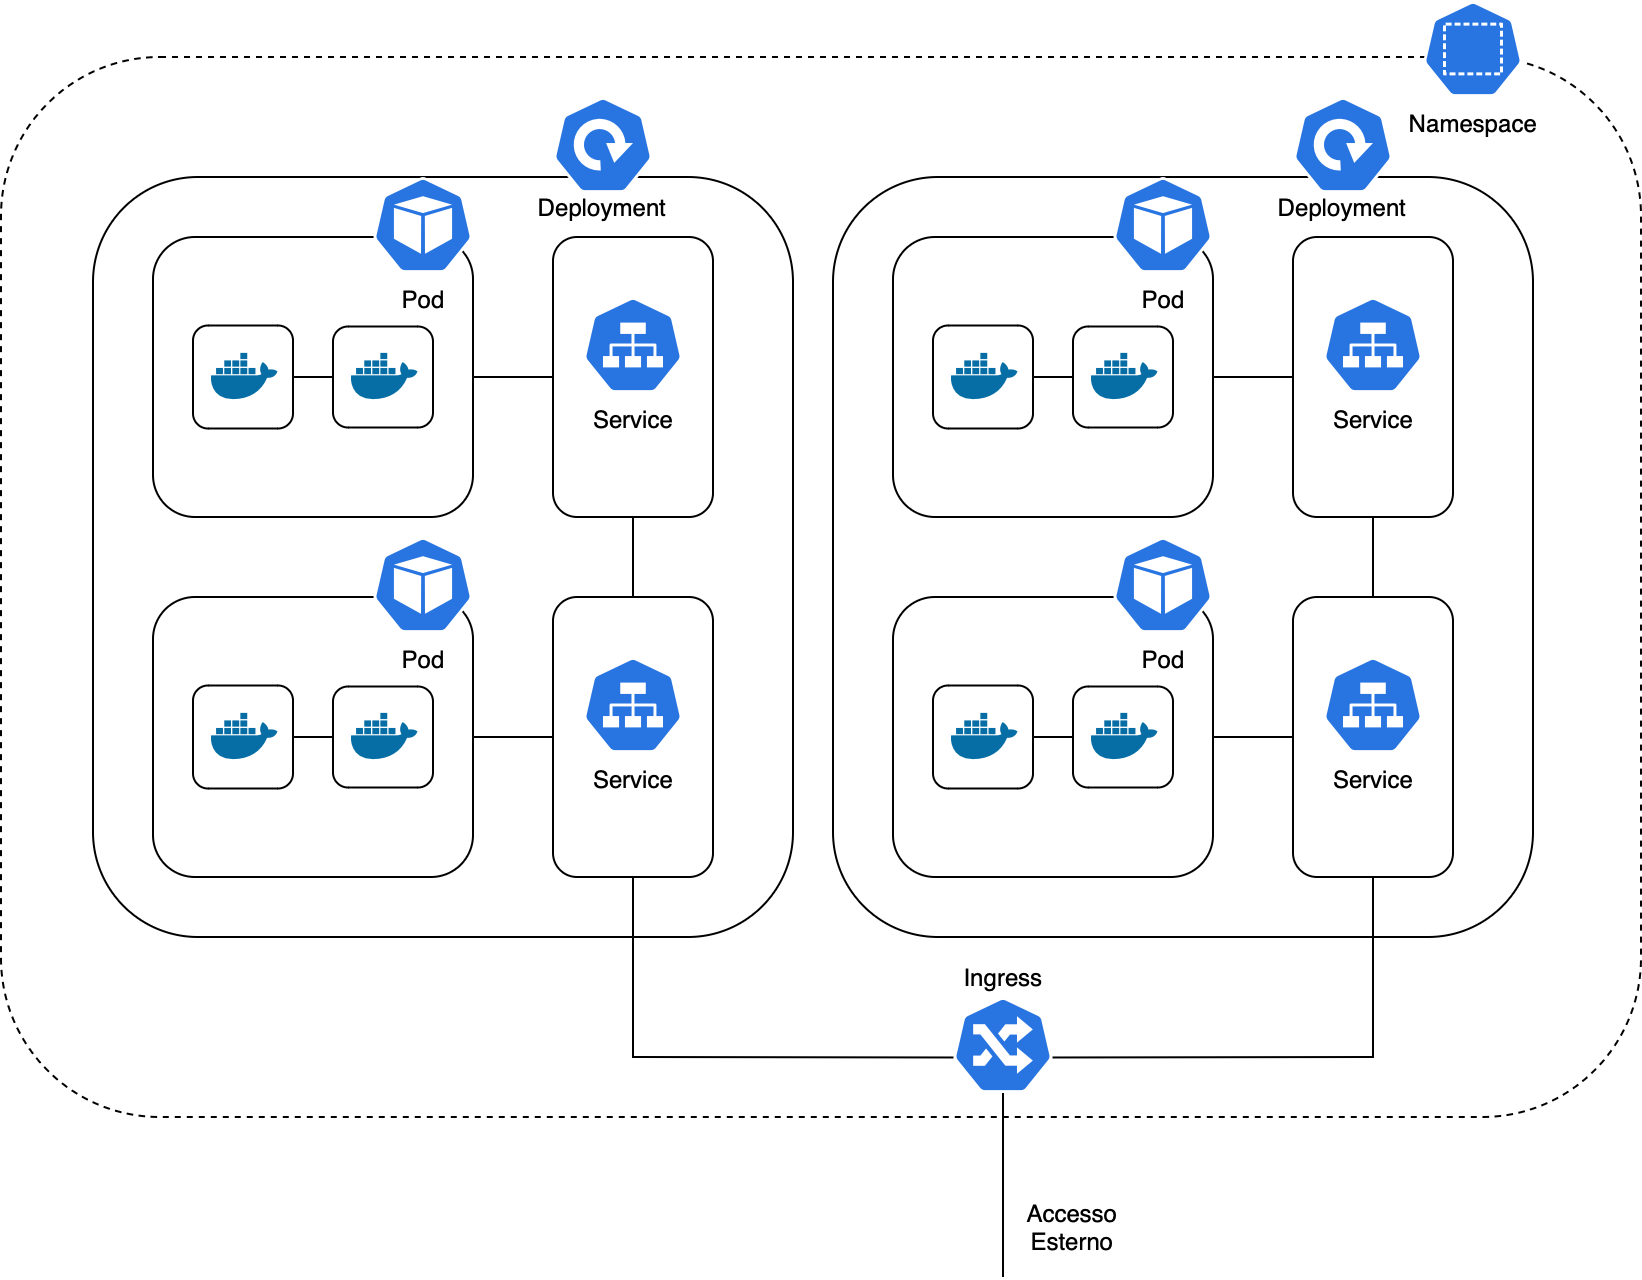
\includegraphics[width=1\linewidth]{immagini/capitolo2/kube_objects.png}
    \caption{Gerarchia e organizzazione delle risorse di Kubernetes.}
    \label{fig:kube_objects}
\end{figure}

\section{Istio}
 Per \textit{Service Mesh} si intende un livello di infrastruttura dedicato che gestisce la comunicazione tra servizi in un sistema distribuito. Questo livello può offrire una serie di funzionalità chiave, come il bilanciamento del carico, la gestione delle reti, la sicurezza e l'osservabilità dei dati, senza che siano gli sviluppatori delle applicazioni ad occuparsene in prima persona.

Tra le tecnologie nativamente integrate con Kubernetes è presente \textit{Istio}\footnote{https://istio.io}, un framework open-source per la gestione dei service mesh. \textit{Istio} fornisce strumenti avanzati per il monitoring, la tracciabilità, la sicurezza e il controllo del traffico tra i servizi. Attraverso una serie di proxy distribuiti in modo uniforme nell'ambiente, Istio riesce a intercettare e gestire il traffico di rete tra microservizi.

\subsection{Caratteristiche di Istio}
Essendo uno degli strumenti più avanzati nel suo campo, Istio offre una serie di caratteristiche distintive:

\begin{itemize}
\item \textbf{Tracciabilità e osservabilità:} Istio permette di ottenere dettagliate informazioni sul traffico, che poi possono essere utilizzati per la diagnosi di problemi nei servizi distribuiti.
\item \textbf{Controllo del traffico:} Attraverso regole e configurazioni dettagliate, Istio può determinare come il traffico viene indirizzato tra servizi, permettendo, ad esempio, un rilascio graduale o un test A/B.
\item \textbf{Sicurezza:} Istio fornisce meccanismi di autenticazione, autorizzazione e crittografia del traffico, garantendo che le comunicazioni tra servizi avvengano in modo sicuro.
\item \textbf{Bilanciamento del carico:} Oltre a semplici strategie round-robin, Istio supporta bilanciamenti più complessi basati su vari parametri e metriche.
\end{itemize}

\subsection{Componenti di Istio}

Istio è composto da due componenti principali che insieme forniscono tutte le sue funzionalità:
\begin{itemize}
    \item \textit{Istiod:} il \textit{Control Plane} della rete Service Mesh Istio
    \item \textit{Proxy Envoy:} il \textit{Data Plane} della rete Service Mesh Istio
\end{itemize}

Entrambi i componenti sono illustrati nei due paragrafi successivi.

\subsubsection{Istiod}

Istiod rappresenta il punto centrale di controllo per l'orchestrazione della Service Mesh. 
Istiod agisce da \myenquote{cervello} centrale, ricevendo configurazioni da file di tipo \texttt{yaml}, e traducendole in un formato comprensibile per il corretto funzionamento della rete. Oltre a questo, Istiod monitora continuamente l'intera mesh per assicurarsi che lo stato attuale del sistema sia conforme alle configurazioni fornite. Se ci sono discrepanze, ad esempio a causa di un guasto o di una modifica non autorizzata, Istiod interviene per correggere la situazione, garantendo così l'integrità e la sicurezza dell'intera mesh.

Nell'ambito di un'architettura di microservizi, è fondamentale garantire coerenza, sicurezza e visibilità su tutte le operazioni tra servizi. Istiod gioca un ruolo chiave in questo scenario, fornendo le seguenti funzionalità principali:

\begin{itemize}
    \item \textbf{Configurazione:} Istiod è responsabile per distribuire la configurazione a tutti i proxy Envoy presenti nella mesh. Ciò significa che ogni cambiamento o aggiornamento delle politiche, regole o configurazioni può essere propagato attraverso Istiod in maniera efficiente e sincronizzata.
    
    \item \textbf{Discovery Service:} Il componente offre un servizio di discovery per i proxy Envoy, permettendo loro di conoscere i servizi presenti all'interno della mesh e di ottenere le informazioni necessarie per il routing e il bilanciamento del carico.
    
    \item \textbf{Gestione delle Certificazioni:} Istiod gestisce anche la certificazione e la rotazione delle chiavi, assicurando che le comunicazioni tra i servizi siano crittografate e sicure. Questa funzionalità garantisce che la Service Mesh aderisca ai più alti standard di sicurezza.
    
    \item \textbf{Validazione:} Ogni volta che una nuova configurazione viene introdotta nella mesh, Istiod la valida per assicurarsi che non ci siano conflitti o errori che potrebbero compromettere il funzionamento del sistema.
    
    \item \textbf{Osservabilità:} Istiod fornisce strumenti e metriche per monitorare il comportamento e le performance della Service Mesh, permettendo agli operatori di avere una visione chiara dello stato del sistema.
\end{itemize}


\subsubsection{Proxy Envoy}

Envoy\footnote{https://www.envoyproxy.io} è un moderno proxy ad alte prestazioni progettato per applicazioni cloud-native. Sviluppato inizialmente da Lyft e ormai incluso da anni come parte integrante della rete Service Mesh Istio, funge da data plane all'interno della Service Mesh, gestendo il traffico tra i servizi e applicando le politiche e regole definite attraverso Istiod.

Le principali caratteristiche e funzionalità offerte da Envoy includono:

\begin{itemize}
    \item \textbf{Bilanciamento del Carico Dinamico:} Envoy supporta una serie di algoritmi di bilanciamento del carico e può adattarsi dinamicamente alle variazioni del sistema, come l'aggiunta o la rimozione di servizi.
    
    \item \textbf{Filtri:} Envoy offre un sistema di filtri estremamente flessibile che può essere utilizzato per manipolare e osservare il traffico in ingresso e in uscita. Ciò consente, ad esempio, di implementare funzionalità di rate limiting, logging e accesso condizionato.
    
    \item \textbf{Sicurezza:} Envoy può gestire connessioni TLS, fornendo crittografia end-to-end e garantendo che le comunicazioni tra servizi siano protette. Inoltre, in combinazione con Istiod, può effettuare autenticazioni mutue tra i servizi, rafforzando ulteriormente la sicurezza dell'intero sistema.
    
    \item \textbf{Osservabilità:} Analogamente a Istiod, anche Envoy fornisce metriche dettagliate sul traffico, latenza, errori e altro ancora, dando una visione completa del comportamento del traffico all'interno della mesh.
\end{itemize}


Il proxy Envoy è anche definito \textit{Sidecar} in quanto, quando aggiunto al sistema, Istiod modifica il deployment in modo da posizionare il proxy dentro un pod, accanto ad ogni container, ed esegue delle manipolazioni tramite la CNI (Container Networking Interface) per intercettare il traffico in ingresso ed in uscita.
\paragraph{Inserimento di Envoy in un deployment}
L'inserimento di Envoy nella rete mesh funziona tramite un meccanismo chiamato \textit{iniezione}. Per rendere possibile l'iniezione, è possibile agire su due livelli:
\begin{itemize}
\item \textbf{Livello namespace:} È possibile, sia all'atto di creazione, sia successivamente, etichettare un namespace in modo da attivare automaticamente l'iniezione di Envoy per tutti i pod che verranno creati in quel namespace. Questo può essere ottenuto applicando al namespace l'etichetta \texttt{istio-injection=enabled}, o richiedendo l'iniezione di una specifica revisione di Istio (che deve essere dotata di una specifica etichetta) tramite l'applicazione della stessa etichetta al namespace, seguendo il preciso schema \verb|istio.io/rev: <nome etichetta>|. Una volta impostate le etichette corrette, ogni pod creato nel namespace avrà automaticamente un proxy Envoy iniettato come sidecar. Questo livello di iniezione è particolarmente utile quando si desidera che tutti i servizi in un particolare namespace facciano parte della rete mesh, senza dover configurare manualmente ogni singolo pod.
\item \textbf{Livello pod:} Anche se un namespace è etichettato per l'iniezione automatica, è possibile sovrascrivere questo comportamento per singoli pod, utilizzando annotazioni specifiche nel loro deployment o nelle definizioni del pod. Questo può essere utile per escludere specifici pod dall'avere un proxy Envoy o, al contrario, per includere un pod in un namespace altrimenti escluso. L'annotazione \texttt{sidecar.istio.io/inject} può essere utilizzata per attivare (\myenquote{true}) o disattivare (\myenquote{false}) l'iniezione a livello di pod.

\end{itemize}
La Figura \ref{fig:envoy} mostra come i proxy Envoy siano dispiegati \myenquote{a fianco} dei servizi, consentendo quindi di intercettarne e gestirne il traffico.

\begin{figure}[h]
    \centering
    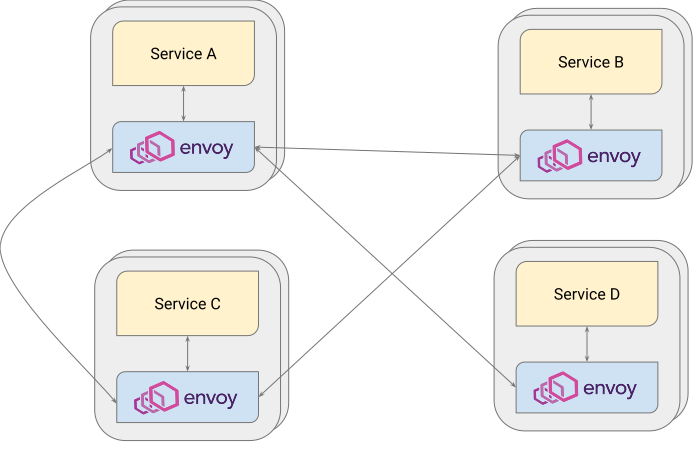
\includegraphics[width=1\linewidth]{immagini/capitolo2/envoy.png}
    \caption{Intercettazione del traffico dati da parte del proxy Envoy \cite{life_of_a_request}.}
    \label{fig:envoy}
\end{figure}


\subsection{Access Logging}

In un'era dominata dalla complessità delle applicazioni e dalla crescente necessità di trasparenza nelle operazioni digitali, monitorare e comprendere il comportamento del traffico diventa essenziale per garantire prestazioni, sicurezza e affidabilità. L'access logging, o registrazione degli accessi, è una pratica proposta come soluzione per tale problema. Questa pratica consiste nel registrare dettagliatamente ogni interazione tra un utente o un servizio e un sistema informatico. In architetture modulari e distribuite, come i microservizi, l'access logging consente di monitorare e registrare (sotto forma di log) le interazioni occorse tra i microservizi di un'applicazione ed il loro esito.

Nella rete service mesh Istio, il proxy Envoy può essere configurato per effettuare access logging, per registrare metriche riguardanti le interazioni tra le applicazioni e i servizi in un ecosistema informatico. Questi strumenti permettono di catturare, in tempo reale, informazioni dettagliate su ogni richiesta e risposta scambiata tra i servizi, facilitando così la diagnosi di problemi, l'analisi delle prestazioni e la gestione proattiva delle potenziali minacce.

All'interno di Envoy, il sistema di access logging è progettato per essere altamente configurabile. È possibile decidere quali informazioni vengono registrate, il formato in cui vengono presentate e la destinazione dei log generati. Ad esempio, è possibile catturare dettagli come l'intestazione HTTP, il corpo della richiesta, i tempi di risposta e molte altre informazioni che possono essere essenziali per la diagnosi di problemi, l'analisi delle prestazioni o la semplice revisione delle operazioni di rete.

\subsection{Integrazione con Kubernetes}

\textit{Istio} è nativamente supportato da \textit{Kubernetes}. Può infatti essere installato come un set di componenti all'interno di un cluster Kubernetes, e può automaticamente scoprire e gestire il traffico tra i pod. Questo rende particolarmente facile e potente l'uso combinato di Kubernetes e Istio per gestire applicazioni distribuite in modo scalabile e sicuro.

\section{Lo stack ELK}

Lo stack ELK, composto da ElasticSearch\footnote{https://www.elastic.co/elasticsearch/}, Logstash\footnote{https://www.elastic.co/logstash/} e Kibana\footnote{https://www.elastic.co/kibana/}, fornisce una soluzione consolidata per l'analisi e la visualizzazione dei dati, particolarmente adatta a log e dati di monitoraggio. La combinazione di ElasticSearch, Logstash e Kibana fornisce infatti un supporto flessibile per raccogliere, indicizzare e visualizzare dati in tempo reale. Lo stack ELK può essere esteso aggiungendo anche il collettore di log Filebeat, ad esempio per rendere più efficiente il processo di collezione dei log in ambienti multi-nodo.

\subsection{ElasticSearch}

ElasticSearch rappresenta uno degli strumenti più avanzati nel panorama dei motori di ricerca e analisi. Basato su Apache Lucene, framework per la ricerca full-text, ElasticSearch è stato sviluppato per soddisfare esigenze avanzate di ricerca, analisi e gestione di enormi volumi di dati in tempo reale.

Per una comprensione approfondita delle potenzialità e del funzionamento di ElasticSearch, è fondamentale introdurre alcuni concetti cardine che ne caratterizzano l'architettura:

\paragraph{Documento}
In ElasticSearch, un documento è l'unità fondamentale di informazione che può essere indicizzata. Un documento rappresenta l'unità di informazione fondamentale su cui ElasticSearch opera e può essere assimilato a un record in un database relazionale. Tuttavia, a differenza di un record tradizionale, un documento in ElasticSearch è in formato JSON e può contenere dati multivariati, quali testo, numeri, date e array. Ogni documento all'interno di un indice è identificato da un ID univoco, che permette di recuperarlo, modificarlo o eliminarlo con facilità. A differenza dei tradizionali database relazionali, dove un record deve aderire rigidamente a uno schema predefinito, in ElasticSearch ogni documento all'interno di un indice può avere una propria struttura, rendendo il sistema molto più flessibile e adattabile a vari scenari.


\paragraph{Indice}
Nel contesto di ElasticSearch, l'indice rappresenta una collezione omogenea di documenti che condividono specifiche caratteristiche o attributi. Questa definizione può essere assimilata alla struttura di una tabella in un sistema di database relazionale. Gli indici in ElasticSearch sono identificati da un nome univoco e possono essere creati, eliminati e configurati dinamicamente. Quando si crea un indice, è possibile definire una serie di impostazioni e mappature che determinano come i documenti e i loro campi sono memorizzati e indicizzati.


\paragraph{Indicizzazione}
Il processo di indicizzazione inizia quando un documento viene inviato ad ElasticSearch. Il documento, attraverso un componente denominato \myenquote{analyzer}, viene smembrato e trasformato in una serie di token. Questi analyzer sono costituiti da tokenizer e token filter. Mentre il tokenizer segmenta il testo in token basandosi su specifici delimitatori, i token filter si occupano della loro elaborazione (per esempio, conversione in minuscolo, eliminazione di parole comuni). Al termine dell'analisi, i token sono inseriti in una struttura chiamata \myenquote{inverted index}, ottimizzata per garantire ricerche veloci ed efficienti.

\paragraph{Elastic Common Schema}\label{subsubsect:ECS}
L'Elastic Common Schema (ECS) rappresenta uno standard nella definizione dei campi per i dati indicizzati su ElasticSearch. Nasce dalla necessità di avere una struttura uniforme dei dati, permettendo alle organizzazioni di semplificare la correlazione, la visualizzazione e l'analisi dei dati provenienti da fonti diverse. Grazie all'ECS, è possibile sfruttare al meglio gli strumenti offerti dalla suite Elastic, come Kibana, per creare visualizzazioni coerenti e interattive. Inoltre, l'ECS facilita l'integrazione di diverse soluzioni e fonti di dati in un ecosistema Elastic unificato, garantendo che le informazioni siano presentate in un formato comune e facilmente comprensibile.


\subsubsection{Caratteristiche distintive di ElasticSearch}

ElasticSearch è un motore di ricerca, che offre una serie di funzionalità avanzate, quali:

\begin{itemize}
\item\textbf{Scalabilità Orizzontale:} La struttura di ElasticSearch consente una facile espansione aggiungendo nodi supplementari al cluster, garantendo una gestione efficace di grandi volumi di dati e traffico.
\item\textbf{Ricerca in Tempo Reale:} L'efficienza del suo sistema di indicizzazione permette a ElasticSearch di fornire risultati di ricerca quasi in tempo reale, con latenze misurabili in millisecondi.
\item\textbf{Analisi dei Dati:} Oltre alla ricerca, ElasticSearch si distingue per le sue capacità analitiche, permettendo agli utenti di trarre intuizioni e conoscenze dai dati in tempo reale.
\item\textbf{Flessibilità:} La sua architettura è progettata per gestire sia dati strutturati che non strutturati e supporta una vasta gamma di formati, tra cui JSON e XML.
\end{itemize}


\subsection{Logstash}

Logstash è un potente strumento per la raccolta, l'elaborazione e l'invio di log ed eventi di dati ad altre piattaforme come ElasticSearch. Concepito per risolvere problemi complessi legati all'ingestione di dati, e distribuito come software open source, Logstash è stato ampiamente adottato grazie alla sua modularità e capacità di integrarsi con svariate fonti e destinazioni di dati.

\subsubsection{Funzionamento}

\paragraph{Input Plugins}
Logstash può ricevere dati da molteplici fonti, grazie ai suoi plugin di input. Che si tratti di log di sistema, flussi di eventi o dati provenienti da database, questi plugin facilitano l'ingestione di dati da svariate origini.

\paragraph{Filter Plugins}
Una volta che i dati sono acquisiti, Logstash offre una serie di plugin di filtraggio per elaborarli. Questi plugin permettono di arricchire, modificare o trasformare i dati in base alle esigenze specifiche.

\paragraph{Output Plugins}
Dopo l'elaborazione, i dati possono essere inviati a diverse destinazioni. Grazie ai plugin di output, Logstash può inviare dati a piattaforme come ElasticSearch, file, metriche, servizi cloud e molte altre soluzioni.

\paragraph{Performance e Scalabilità}

Con una progettazione orientata alla performance, Logstash può gestire volumi significativi di dati. La sua architettura supporta una scalabilità orizzontale, consentendo di distribuire l'elaborazione su più istanze e nodi.

\paragraph{Applicazioni e Casistiche d'Uso}

Logstash non si limita a essere un semplice strumento di ingestione di log. Le sue capacità di filtraggio e trasformazione rendono possibile l'uso in diversi scenari, tra cui:

\begin{enumerate}
\item \textbf{Analisi e Monitoraggio:} Integrando Logstash con ElasticSearch e Kibana, gli utenti possono creare dashboard e visualizzazioni avanzate per monitorare applicazioni, infrastrutture e servizi.
\item \textbf{Allerta e Notifiche:} Logstash può essere configurato per rilevare pattern specifici nei dati e generare allerte in tempo reale.
\item \textbf{Archiviazione Centralizzata:} Per le casistiche che necessitano di un sistema centralizzato di archiviazione dei log, Logstash offre soluzioni robuste e affidabili.
\end{enumerate}

\subsection{Kibana}

Kibana è una piattaforma di visualizzazione e dashboarding per ElasticSearch. Essa fornisce funzionalità di ricerca in tempo reale e offre la possibilità di creare visualizzazioni grafiche avanzate basate sui dati immagazzinati in ElasticSearch. Essendo l'ultimo componente dell'ELK Stack, Kibana completa il ciclo di ingestione, elaborazione e visualizzazione dei dati.

Le caratteristiche principali di Kibana sono le seguenti:

\paragraph{Interfaccia Utente Intuitiva}

Kibana è stata progettata con un'attenzione particolare all'esperienza dell'utente. La sua interfaccia grafica consente anche agli utenti meno esperti di esplorare e visualizzare i dati senza la necessità di conoscere linguaggi di query complessi.

\paragraph{Visualizzazioni Avanzate}

Dai semplici grafici a barre e linee alle mappe geospaziali, Kibana offre una vasta gamma di opzioni per visualizzare i dati. Gli utenti possono personalizzare le visualizzazioni in base alle proprie esigenze e integrarle in dashboard interattive.

\paragraph{Integrazione con ElasticSearch}

La profonda integrazione con ElasticSearch consente a Kibana di fornire funzionalità di ricerca avanzata, facilitando l'esplorazione dei dati e la creazione di visualizzazioni basate su query specifiche.


\subsection{Filebeat}

Filebeat\footnote{https://www.elastic.co/beats/filebeat} è un distributore di log che monitora i file e le directory specificate, cattura gli eventi e li invia per l'elaborazione o direttamente ad ElasticSearch. Fa parte della famiglia di prodotti Beats di Elastic e si integra nativamente con lo stack ELK, fornendo una soluzione per raccogliere dati da file di log, flussi di log di sistema o qualsiasi sorgente di dati basata su file. Di seguito, le principali caratteristiche di Filebeat:

\begin{itemize}
\item \textbf{Leggerezza:} Filebeat è progettato per essere leggero e avere un impatto minimo sulle risorse di sistema. Può essere eseguito su server, macchine virtuali e persino dispositivi IoT.
\item \textbf{Resilienza e affidabilità:} Filebeat ha la capacità di tenere traccia della posizione dei file di log letti. In caso di interruzione, può riprendere la lettura dal punto in cui si era interrotto, garantendo che non vengano persi log.
\item \textbf{Moduli integrati:} Filebeat offre moduli preconfigurati per diversi tipi di log, come Kubernetes, Apache, Nginx, e molti altri, semplificando la raccolta, la trasformazione e l'invio di dati specifici a ElasticSearch o Logstash.
\item \textbf{Integrazione flessibile:} Mentre l'integrazione diretta con ElasticSearch è comune, Filebeat può anche inviare dati a Logstash per ulteriori elaborazioni o trasformazioni prima di indicizzarli in ElasticSearch.
\end{itemize}

\subsection{Utilizzo con Kubernetes}
Se utilizzato in un cluster gestito con Kubernetes, lo stack ELK può fornire un supporto per il monitoraggio e l'analisi dei log. 
ElasticSearch può essere utilizzato per immagazzinare log da vari pods e servizi all'interno del cluster. Logstash può raccogliere questi log, eventualmente trasformarli o arricchirli, e infine inviarli a ElasticSearch per l'indicizzazione. Kibana, infine, può essere utilizzato dagli amministratori del sistema o dai team di sviluppo per analizzare questi log, identificare problemi o tendenze e prendere decisioni informate. Con l'aggiunta di Filebeat, è possibile raccogliere i log garantendo la minima occupazione delle risorse.

\section{yRCA}
yRCA\footnote{https://github.com/di-unipi-socc/yRCA} è uno strumento per l'analisi delle cause scatenanti di fallimenti osservati in applicazioni basate su microservizi. L'analisi effettuata su yRCA, nel senso che non solo vengono identificate le possibili cause di un fallimento, ma viene anche fornita una spiegazione di come tali cause possano essere risultate nel fallimento osservato.

yRCA ricerca le cause di un fallimento processando i log dei microservizi di un'applicazione, assumendo che tali microservizi emettano log per tracciare i loro fallimenti, le interazioni con gli altri servizi ed il loro esito. Sotto tale assunzione, le possibili cause di un fallimento sono identificate considerando otto scenari distinti: cinque di natura ricorsiva, associati a catene di fallimenti, e tre come casi di base, legati alle cause principali degli errori. Le cause possibili di errore di yRCA sono:

\begin{enumerate}

\item \textbf{Errore interno di un'istanza di servizio invocata:} Il fallimento loggato da un servizio A, conseguente a un'interazione non riuscita o scaduta con l'entità B, potrebbe essere risultante da un errore interno dell'entità B. In tale contesto, l'approccio si basa sull'errore interno di B per fornire una spiegazione.

\item \textbf{Interazione fallita di un’istanza di servizio invocata:} Il fallimento loggato da un servizio A potrebbe essere dovuto al fallimento dell'interazione con un servizio B, che a sua volta potrebbe essere causato da un'interazione non riuscita di B con C. Dopo aver determinato la sequenza di guasti a cascata C → B → A, l'approccio utilizza le informazioni del guasto di B per spiegare il fallimento di A.

\item \textbf{Interazione scaduta di un'istanza di servizio invocata:} Il fallimento loggato da un servizio A è stato indotto da un evento analogo in un servizio B, a seguito di un timeout nell'interazione di B con un servizio C. Una volta identificata la sequenza di timeout C → B → A, si fa riferimento al timeout di B per elaborare una spiegazione.

\item \textbf{Irraggiungibilità di un servizio invocato da un'istanza di servizio:} Il fallimento loggato da un servizio A è risultato da un timeout in un servizio B, a causa di un'interazione fallita di B. Diversamente dai precedenti casi, si considera l'ipotesi che la richiesta trasmessa da B non sia stata accettata da un servizio C, provocando quindi il fallimento per timeout. Dopo aver identificato la sequenza di guasti C → B → A, si fa riferimento al registro del timeout in B per spiegare il fallimento.

\item \textbf{Irraggiungibilità di un'istanza di servizio invocata:} Il fallimento loggato da un servizio A è nato da una richiesta non ricevuta durante l'interazione tra A e un servizio B. In questo contesto, si fa riferimento al fatto che B era irraggiungibile per fornire una spiegazione.

\item \textbf{Errore interno di un servizio:} Questa situazione interpreta un fallimento loggato da un servizio, indicando lo stesso servizio come l'origine dell'errore. La procedura ricorsiva si conclude qui.

\item \textbf{Temporanea irraggiungibilità di un servizio:} Questa situazione interpreta i fallimenti loggati da un servizio, rivelando che il servizio era temporaneamente irraggiungibile, poiché aveva registrato determinate informazioni in precedenza. La procedura ricorsiva si conclude.

\item \textbf{Servizio non avviato:} Quest'ultima situazione illustra i fallimenti loggati da un servizio, rivelando che il servizio non ha mai registrato informazioni. La procedura ricorsiva si conclude, riconoscendo che tale servizio potrebbe non essere mai stato avviato.
\end{enumerate}

\subsection{Ricostruzione delle interazioni}
Per ricostruire le interazioni, yRCA utilizza un campo chiamato \textit{request\_id}. Questo campo contiene un UUID\cite{leach_uuid_urn}, ovvero un identificativo univoco generato casualmente con lo scopo di correlare log riferenti la medesima interazione. Quando un servizio inizia un'interazione con un altro, il proxy Envoy associato al servizio chiamante genera nei propri log un UUID che viene trasmesso al proxy del servizio ricevente, e riferito a quella specifica interazione. Man mano che l'interazione si muove attraverso vari servizi o componenti, questo UUID viene trasmesso lungo la catena. Ciò permette di correlare tutti i log associati ad una singola interazione, indipendentemente da dove questi vengano generati.